\documentclass[11pt]{style/memo}

\usepackage{tikz}
    \usetikzlibrary{arrows.meta}
\usepackage{amsmath, amssymb, mathtools}
\usepackage{cancel}
\usepackage{multirow}
\usepackage{colortbl, xcolor}

\title{Parallel 2D Physics}
\author{Kevin J. Dugan}
\date{November 14, 2022}

\begin{document}
\maketitle

\section{Quadrilateral Mesh}
Let's look at the discretization and basis functions for a 2D mesh
typical for physics simulations. We'll use quadrilateral/hexahedral
elements because they offer a direct extension from 1D elements through
tensor products. As usual, we assume that the simulation domain is
discretized using a non-overlapping set of $N$ cells $\Omega$. For a 2D
domain, we can structure the discretization as

\begin{equation*}
    \Omega = \begin{bmatrix}
        (x,y)_0 & (x,y)_1 & (x,y)_2 & (x,y)_3 \\
        (x,y)_4 & (x,y)_5 & (x,y)_6 & (x,y)_2 \\
        \vdots & \vdots & \vdots & \vdots \\
        (x,y)_{M-3} & (x,y)_{M-2} & (x,y)_{M-1} & (x,y)_M
    \end{bmatrix}
\end{equation*}

where there are $M+1$ vertices in the mesh. Realize that vertices may appear
more than once in $\Omega$ for those cells which share edges. Each row in
$\Omega$ represents the vertices of a cell and the shape of $\Omega$ is
$(\mathrm{N}_\mathrm{cells} \times 4)$. 

The typical data structure for $\Omega$ would have a level of indirection
by defining an ordered set of spatial points, then $\Omega$ would be defined
by a connectivity matrix where each entry would be an index referencing a
spatial point. I'll mention here that the ordering of vertices for a cell
follow a counter-clockwise ordering, which will aid in transforming cells
to a reference element during matrix assembly.

\section{2D Basis Functions}
We'll start with a definition of hierarchical basis functions ($\vec{b}_i$) on a
1D reference element ($\mathcal{E}$). The choice of basis functions has an
important effect on the condition number of the assembled matrix, which we'll
leave for another time. The important charactaristics we need are the linear
functions are 1 at the element edges and the ``bubble'' functions for higher
order functions are zero at the element edges. The functions should also
form a complete basis for the polynomial space defined over the element,
but are not required to be orthogonal.

\begin{equation}
    \label{eq:hier1d}
    \vec{b}(\xi) = \frac{1}{2} \begin{bmatrix}
        1-\xi \\
        1+\xi \\
        2 \left( 1-x^2 \right) \\
        \frac{7\sqrt{7}-10}{8} \left( 1 - 3\xi - \xi^2 + 3\xi^3\right)
    \end{bmatrix}
    \qquad
    \xi \in [-1,1]
\end{equation}

The functions from Equation~\ref{eq:hier1d} are visualized in Figure~\ref{fig:hier1d}

\begin{figure}[h]
    \centering
    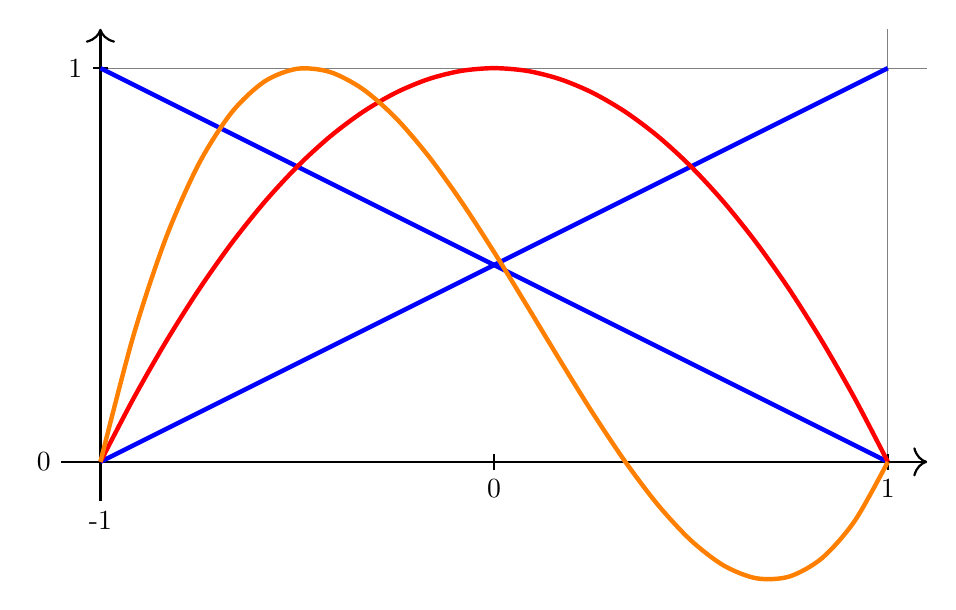
\begin{tikzpicture}
        % Axes
        \draw[gray] (-5,5) -- (5.5,5);
        \draw[gray] (5,0) -- (5,5.5);
        \draw[thick, -{>[scale=1.5]}] (-5.5,0) node[anchor=east] {0} -- (5.5,0);
        \draw[thick] (0,0.1) -- (0,-0.1) node[anchor=north] {0};
        \draw[thick] (5,0.1) -- (5,-0.1) node[anchor=north] {1};
        \draw[thick, -{>[scale=1.5]}] (-5,-0.5) node[anchor=north] {-1} -- (-5,5.5);
        \draw[thick] (-4.9,5) -- (-5.1,5) node[anchor=east] {1};

        % \draw
        \draw[ultra thick, domain=-5:5, smooth, variable=\x, blue] plot ({\x}, {5.0*0.5*(1.0-\x/5.0)});
        \draw[ultra thick, domain=-5:5, smooth, variable=\x, blue] plot ({\x}, {5.0*0.5*(1.0+\x/5.0)});
        \draw[ultra thick, domain=-5:5, smooth, variable=\x, red] plot ({\x}, {5.0*(1.0-(\x/5.0)*(\x/5.0))});
        \draw[ultra thick, domain=-5:5, smooth, variable=\x, orange] plot ({\x}, {5.0*0.5*1.065*(1.0-3.0*(\x/5.0)-(\x/5.0)*(\x/5.0)+3.0*(\x/5.0)*(\x/5.0)*(\x/5.0))});
    \end{tikzpicture}
    \caption{Hierarchical Lagrangian basis functions up to order 3}
    \label{fig:hier1d}
\end{figure}

In the following discussions, we'll talk about \emph{support points} which are locations
that are non-zero for the basis functions. Referring to Figure~\ref{fig:hier1d}, the linear
basis functions have support points on the edge of the reference element and the higher
order functions have support points in the interior of the reference element. Support
points will correspond to \emph{Degrees of Freedom} (DoFs) in the assembled linear system.

Given a 2D reference element ($\mathcal{E}^2 = \{x,y|x,y\in \left[-1,1\right]\}$), the
2D basis functions can be defined through a tensor product of the 1D basis functions.
The tensor product in this context can be thought of an outer product ($\vec{a}\vec{b}^{\,T}$) flattened
into a rank 1 vector. Note that this only applies on quadrilateral/hexahedral elements;
triangular based elements don't have this property.

\begin{equation}
    \vec{b}(\xi,\eta) = \vec{b}(\xi) \otimes \vec{b}(\eta)
\end{equation}

Expanding the hierarchical elements defined in Equation~\ref{eq:hier1d}, only up to
quadratic order for brevity, yields the following

\begin{equation}
    \label{eq:hier2d}
    \vec{b}(\xi,\eta) = \frac{1}{4} \begin{bmatrix}
        & \cellcolor{blue!20!white} (1-\xi)(1-\eta)     & \cellcolor{blue!20!white} (1-\xi)(1+\eta)     & \cellcolor{green!20!white} 2(1-\xi)(1-\eta^2) \\
        & \cellcolor{blue!20!white} (1+\xi)(1-\eta)     & \cellcolor{blue!20!white} (1+\xi)(1+\eta)     & \cellcolor{green!20!white} 2(1+\xi)(1-\eta^2) \\
        & \cellcolor{green!20!white} 2(1-\xi^2)(1-\eta) & \cellcolor{green!20!white} 2(1-\xi^2)(1+\eta) & \cellcolor{red!20!white} 4(1-\xi^2)(1-\eta^2)
    \end{bmatrix}
\end{equation}

where regions highlighted with light blue ({\color{blue!20!white}\rule{1em}{1em}})
correspond to linear shape functions which have support points on vertices. Regions
highlighted with light green ({\color{green!20!white}\rule{1em}{1em}}) correspond
to shape functions which have support points on edges. Regions highlighted with light
red ({\color{red!20!white}\rule{1em}{1em}}) bubble functions which have support points
in the interior of the element.

In an abbreviated way (Equation~\ref{eq:hier2d_q3}), we can show the hierarchical bases
functions for a 2D element up to polynomial order 3 by denoting the order $Q_\mathrm{n}$
and denoting the type of function with $Q^{\{V,E,B\}}$ for functions which have support
points on the vertices, edges, or interior (bubble).

\begin{equation}
    \label{eq:hier2d_q3}
    \vec{b}(\xi,\eta) = \begin{bmatrix}
        & \cellcolor{blue!20!white}  Q_1^V & \cellcolor{blue!20!white}  Q_1^V & \cellcolor{green!20!white} Q_2^E & \cellcolor{green!20!white} Q_3^E \\
        & \cellcolor{blue!20!white}  Q_1^V & \cellcolor{blue!20!white}  Q_1^V & \cellcolor{green!20!white} Q_2^E & \cellcolor{green!20!white} Q_3^E \\
        & \cellcolor{green!20!white} Q_2^E & \cellcolor{green!20!white} Q_2^E & \cellcolor{red!20!white}   Q_2^B & \cellcolor{red!20!white}   Q_3^B \\
        & \cellcolor{green!20!white} Q_3^E & \cellcolor{green!20!white} Q_3^E & \cellcolor{red!20!white}   Q_3^B & \cellcolor{red!20!white}   Q_3^B
    \end{bmatrix}
\end{equation}

In the assembled linear system, each basis function will be associated with one DoF.
From Equation~\ref{eq:hier2d_q3}, we can calculate the number of DoFs in the system since
there will always be one DoF per vertex, $(q-1)$ DoFs per edge, and $(q-1)^2$ DoFs
per element. The hierarchical shape functions used are shown in Figure~\ref{fig:hier2d}.

\begin{figure}[h]
    \centering
    \begin{subfigure}[b]{0.3\textwidth}
        \centering
        \includegraphics[width=\textwidth]{figures/quadrature2D_000.png}
    \end{subfigure}
    \hfill
    \begin{subfigure}[b]{0.3\textwidth}
        \centering
        \includegraphics[width=\textwidth]{figures/quadrature2D_001.png}
    \end{subfigure}
    \hfill
    \begin{subfigure}[b]{0.3\textwidth}
        \centering
        \includegraphics[width=\textwidth]{figures/quadrature2D_002.png}
    \end{subfigure}

    \begin{subfigure}[b]{0.3\textwidth}
        \centering
        \includegraphics[width=\textwidth]{figures/quadrature2D_004.png}
    \end{subfigure}
    \hfill
    \begin{subfigure}[b]{0.3\textwidth}
        \centering
        \includegraphics[width=\textwidth]{figures/quadrature2D_005.png}
    \end{subfigure}
    \hfill
    \begin{subfigure}[b]{0.3\textwidth}
        \centering
        \includegraphics[width=\textwidth]{figures/quadrature2D_006.png}
    \end{subfigure}

    \begin{subfigure}[b]{0.3\textwidth}
        \centering
        \includegraphics[width=\textwidth]{figures/quadrature2D_008.png}
    \end{subfigure}
    \hfill
    \begin{subfigure}[b]{0.3\textwidth}
        \centering
        \includegraphics[width=\textwidth]{figures/quadrature2D_009.png}
    \end{subfigure}
    \hfill
    \begin{subfigure}[b]{0.3\textwidth}
        \centering
        \includegraphics[width=\textwidth]{figures/quadrature2D_010.png}
    \end{subfigure}
    \caption{Collection of $Q_2$ hierarchical shape functions for a 2D element. Ordering from Equation~\ref{eq:hier2d}}
    \label{fig:hier2d}
\end{figure}

The three bubble functions and a representative edge function for the $Q_3$ elements
are shown in Figure~\ref{fig:hier2d_q3}.

\begin{figure}[h]
    \centering
    \begin{subfigure}[b]{0.49\textwidth}
        \centering
        \includegraphics[width=\textwidth]{figures/quadrature2D_007.png}
    \end{subfigure}
    \hfill
    \begin{subfigure}[b]{0.49\textwidth}
        \centering
        \includegraphics[width=\textwidth]{figures/quadrature2D_011.png}
    \end{subfigure}

    \begin{subfigure}[b]{0.49\textwidth}
        \centering
        \includegraphics[width=\textwidth]{figures/quadrature2D_014.png}
    \end{subfigure}
    \hfill
    \begin{subfigure}[b]{0.49\textwidth}
        \centering
        \includegraphics[width=\textwidth]{figures/quadrature2D_015.png}
    \end{subfigure}
    \caption{Example edge shape function and bubble functions for a $Q_3$ 2D element}
    \label{fig:hier2d_q3}
\end{figure}

\section{Transformation to Reference Element}
We've based this discussion on functions defined on a reference element, which means
that during the system assembly we'll need to map a physical element to the
reference element. We'll stipulate that the physical elements need to have straight
edges so that a bilinear map can be used for the transformation --- curved elements
would require a higher order map for the transformation.

By pure coincidence, the bilinear map for the transformation can be constructed from the
linear basis functions shown in Equation~\ref{eq:hier2d}. Since these are two unrelated
sets of functions, I'll use a different notation so there's less confusion.

\begin{eqnarray*}
    g^0(\xi) = \frac{1 - \xi}{2} \\
    g^1(\xi) = \frac{1 + \xi}{2}
\end{eqnarray*}

Then, the mapping from reference coordinates to physical coordinates for a 1D element
can be expressed as

\begin{equation}
    x(\xi) = g^0(\xi) x_L + g^1(\xi) x_R = \begin{bmatrix}
        g^0(\xi) \\ g^1(\xi)
    \end{bmatrix}^T
    \begin{bmatrix}
        x_0 \\ x_1
    \end{bmatrix}
\end{equation}

The Jacobian for the coordinate transformation will appear during the assembly and is
defined for a 1D change in Equation~\ref{eq:jac_1d}. I'll take advantage of Einstein
summation notation for some of these identities.

\begin{equation}
    \label{eq:jac_1d}
    \mathcal{J}_e = \frac{d x}{d\xi} = \frac{dg^i}{d\xi}x_i
\end{equation}

It's difficult to tell in the 1D case, but we've imposed a left-to-right ordering of
the coordinates and the corresponding ordering for the transformation functions.
It's natural to have a left-to-right ordering in 1D, but in higher dimensions there
is more freedom for the ordering. This ordering will be counter-clockwise
for 2D elements.

\subsection{2D Reference Element Transformation}
For 2D elements, we impose a counter-clockwise ordering of the vertices on an element.
The corresponding transformation function is shown in Equation~\ref{eq:transform2d}

\begin{eqnarray}
    \begin{bmatrix}
        x(\xi,\eta) & y(\xi,\eta)
    \end{bmatrix} = 
    \frac{1}{4}
    \begin{bmatrix}
        (1-\xi)(1-\eta) \\
        (1+\xi)(1-\eta) \\
        (1+\xi)(1+\eta) \\
        (1-\xi)(1+\eta)
    \end{bmatrix}^T
    \begin{bmatrix}
        x_0 & y_0 \\
        x_1 & y_1 \\
        x_2 & y_2 \\
        x_3 & y_3
    \end{bmatrix}
    = \begin{bmatrix}
        g^i(\xi,\eta)x_i &
        g^i(\xi,\eta)y_i
    \end{bmatrix}
    \label{eq:transform2d}
\end{eqnarray}

The Jacobian $\mathcal{J}$ for element $e$ can be defined in the following way

\begin{equation*}
    \mathcal{J}_e = \begin{bmatrix}
        \dfrac{\strut\partial x(\xi,\eta)}{\strut\partial\xi}  & \dfrac{\strut\partial y(\xi,\eta)}{\strut\partial\xi} \\
        \dfrac{\strut\partial x(\xi,\eta)}{\strut\partial\eta} & \dfrac{\strut\partial y(\xi,\eta)}{\strut\partial\eta}
    \end{bmatrix}
    =
    \begin{bmatrix}
        \dfrac{\strut\partial g^i}{\strut\partial\xi}x_i & \dfrac{\strut\partial g^i}{\strut\partial\xi}y_i \\
        \dfrac{\strut\partial g^i}{\strut\partial\eta}x_i & \dfrac{\strut\partial g^i}{\strut\partial\eta}y_i
    \end{bmatrix}
\end{equation*}


We can visualize the transformation of a 2D element in Figure~\ref{fig:transform2d}.

\begin{figure}[h]
\centering
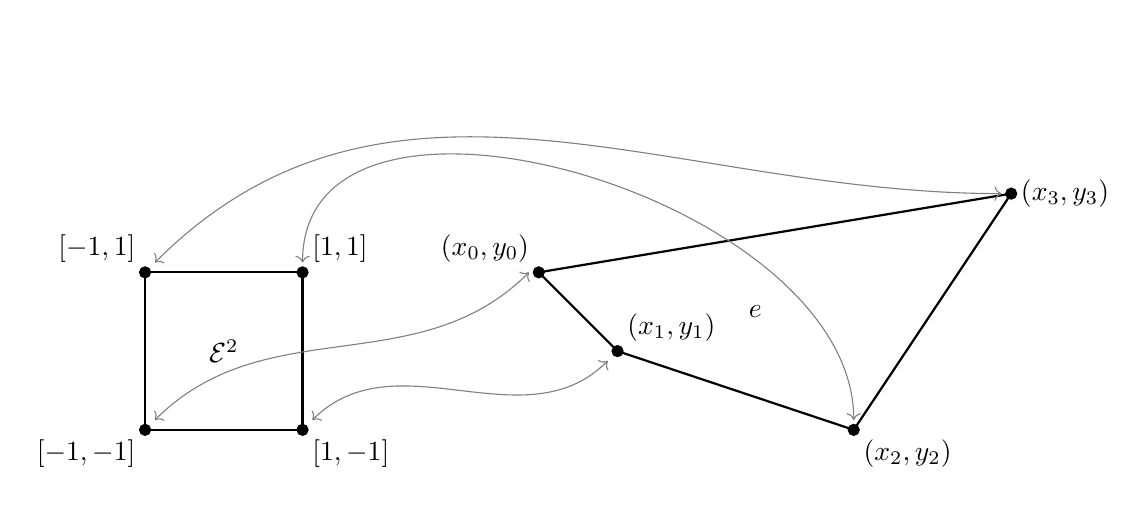
\begin{tikzpicture}[scale=2]
    % Reference Element
    \draw[thick] (0,0) -- (1,0) -- (1,1) -- (0,1) -- (0,0);
    \node at (0.5, 0.5) {$\mathcal{E}^2$};
    % Lower Left
    \draw[fill] (0,0) circle [radius=1pt];
    \node (A) at (0,0) {};
    \node[below left] at (0,0) {$[-1,-1]$};
    % Lower Right
    \draw[fill] (1,0) circle [radius=1pt];
    \node (B) at (1,0) {};
    \node[below right] at (1,0) {$[1,-1]$};
    % Upper Right
    \draw[fill] (1,1) circle [radius=1pt];
    \node (C) at (1,1) {};
    \node[above right] at (1,1) {$[1,1]$};
    % Upper Left
    \draw[fill] (0,1) circle [radius=1pt];
    \node (D) at (0,1) {};
    \node[above left] at (0,1) {$[-1,1]$};

    % Distorted Element
    \draw[thick] (3,0.5) -- (4.5,0) -- (5.5,1.5) -- (2.5,1) -- (3,0.5);
    \node at (3.875,0.75) {$e$};
    % Lower Left
    \draw[fill] (3,0.5) circle [radius=1pt];
    \node (X) at (3,0.5) {};
    \node[above right] at (3,0.5) {$(x_1,y_1)$};
    % Lower Right
    \draw[fill] (4.5,0) circle [radius=1pt];
    \node (Y) at (4.5,0) {};
    \node[below right] at (4.5,0) {$(x_2,y_2)$};
    % Upper Right
    \draw[fill] (5.5,1.5) circle [radius=1pt];
    \node (Z) at (5.5,1.5) {};
    \node[right] at (5.5,1.5) {$(x_3,y_3)$};
    % Lower Left
    \draw[fill] (2.5,1) circle [radius=1pt];
    \node (W) at (2.5,1) {};
    \node[above left] at (2.5,1) {$(x_0,y_0)$};

    % Mapping lines
    \draw[<->, gray] (A.north east) [out=45,in=225] to (W.west);
    \draw[<->, gray] (B.north east) [out=45,in=225] to (X.south west);
    \draw[<->, gray] (C.north)      [out=90,in=90]  to (Y.north);
    \draw[<->, gray] (D.north east) [out=45,in=180] to (Z.west);

\end{tikzpicture}
\caption{Transformation between mesh element and reference element}
\label{fig:transform2d}
\end{figure}

\subsection{Basis function Transformation}
From the variational formulation of whatever system we are solving, we'll need
to assemble a linear system uing a \emph{Change of Variables}. In general, we
will use the following

\begin{equation*}
    \int_\mathrm{E} f(x,y) d\mathrm{E} \Rightarrow \int_\mathcal{E}
    f\left(x(\xi,\eta), y(\xi,\eta)\right)
    \left\lvert J \right\rvert
    d\mathcal{E}
\end{equation*}

Additionally, recall the gradient operation and how the Jacobian relates to
basis functions defined on the reference element.

\begin{equation*}
    \vec{\nabla} b_i(x,y) = \begin{bmatrix}
        \dfrac{\strut\partial b_i(\xi,\eta)}{\strut\partial \xi}\dfrac{\strut\partial \xi}{\strut\partial x} +
        \dfrac{\strut\partial b_i(\xi,\eta)}{\strut\partial \eta}\dfrac{\strut\partial \eta}{\strut\partial x}
        \\
        \dfrac{\strut\partial b_i(\xi,\eta)}{\strut\partial \xi}\dfrac{\strut\partial \xi}{\strut\partial y} +
        \dfrac{\strut\partial b_i(\xi,\eta)}{\strut\partial \eta}\dfrac{\strut\partial \eta}{\strut\partial y}
    \end{bmatrix}^T
    =
    \begin{bmatrix}
        \dfrac{\strut\partial b_i}{\strut\partial \xi} & \dfrac{\strut\partial b_i}{\strut\partial \xi}
    \end{bmatrix}
    \underbrace{
    \begin{bmatrix}
        \dfrac{\strut\partial \xi}{\strut\partial x} & \dfrac{\strut\partial \xi}{\strut\partial y} \\
        \dfrac{\strut\partial \eta}{\strut\partial x} & \dfrac{\strut\partial \eta}{\strut\partial y}
    \end{bmatrix}
    }_{\left(J^{-1}\right)^T}
\end{equation*}

\section{Linear System Assembly}
\subsection{Physics Model}
To illustrate the process for generating a linear system of equations, a linear heat conduction
model (\ref{eq:continuous_model}) is chosen.

\begin{equation}
    \label{eq:continuous_model}
    \begin{gathered}
        -\vec{\nabla}\cdot\left(k(x,y) \vec{\nabla} T \right) = Q, \qquad x,y \in \Omega \\
        \left. \vec{\nabla}T\cdot\vec{n} \right|_{\partial\Omega_N} = 0 \qquad \left. T \right|_{\partial\Omega_D} = T_D,
    \end{gathered}
\end{equation}

\subsection{Spatial Discretization}
The spatial discretization can be acheived through a variational formulation
by left-multiplying a basis vector and integrating over the domain.

\begin{equation*}
    -\int_\Omega \vec{b}_i \vec{\nabla}\cdot\left(k(x,y) \vec{\nabla} T \right)d\Omega = \int_\Omega \vec{b}_i Q d\Omega
\end{equation*}

The first term can be simplified by  using integration by parts (which can be derived from the
product rule for differentiation). The following is referred to as the \emph{weak form} of
(\ref{eq:continuous_model}).

\begin{equation*}
    \int_\Omega k(x,y) \vec{\nabla}\vec{b}_i \cdot \vec{\nabla} T d\Omega - \left. k(x,y)\vec{b}_i\vec{\nabla}T \right|_{\partial\Omega} = \int_\Omega \vec{b}_i Q d\Omega
\end{equation*}

Since the model problem (\ref{eq:continuous_model}) has homogeneous Neumann boundary conditions, the
second term in the above will evaluate to zero and thus will be dropped. If non-homogeneous Neumann
conditions were present, these contributions would appear in the system assembly. To finish the
discretiztion, an approximation must be made for the solution

\begin{equation*}
    T(x) \approx \sum_j T_j b_j(x)
\end{equation*}

Substituting this approximation into the linear system will produce the discretized form of the
linear system (\ref{eq:disc_model})

\begin{equation}
    \label{eq:disc_model}
    \left[ \int_\Omega k(x,y) \vec{\nabla}\vec{b}_i \vec{\nabla}\vec{b}_j^{\,T} d\mathrm{E} \right] \vec{T} = \int_\Omega \vec{b}_i Q d\Omega
\end{equation}

where $\vec{T}$ is a vector of the $\{T_j\}$ coefficients.

The integrals over the whole domain $\Omega$ are computed by summing contributions from each
cell of the discretization.

\begin{equation*}
    \left[ \sum_{\mathrm{E}\in\Omega}\int_\mathrm{E} k(x,y) \vec{\nabla}\vec{b}_i \vec{\nabla}\vec{b}_j^{\,T} d\mathrm{E} \right] \vec{T} = \sum_{\mathrm{E}\in\Omega}\int_\mathrm{E} \vec{b}_i Q d\Omega
\end{equation*}

Now it should become apparent why the previous sections focused on transformations to reference
elements. We can transform the integrals over physical cells to reference cells.

\begin{equation*}
    \left[ \sum_{\mathrm{E}\in\Omega}\int_\mathcal{E} k(\xi,\eta) \vec{\nabla}\vec{b}_i (J^{-1})^T(J^{-1}) \vec{\nabla}\vec{b}_j^{\,T} \left\lvert J \right\rvert d\mathcal{E} \right] \vec{T} = \sum_{\mathrm{E}\in\Omega}\int_\mathcal{E} \vec{b}_i Q \left\lvert J \right\rvert d\mathcal{E}
\end{equation*}

\nocite{segerlind-1984, zienkiewicz-2005, guermond-2000, buluc-2011}
\bibliographystyle{unsrt}
\bibliography{references}

\end{document}